\title{Sample Midterm Exam 1\ifsol\\[4pt]\large Answer Key\fi}
\author{Econ 5030}
\date{}

\begin{document}
\maketitle
\thispagestyle{myheadings}

\section{Preferences}

\noindent Consider an agent with preferences over $X=[0,1]\times[0,1]$ defined as follows: For all $x,x'\in X$,
\[
x \succsim x' \quad\text{if and only if}\quad x_1 \ge x_1' \text{ and } x_2 \ge x_2'.
\]

\begin{description}
\item[1.1] Write the definition of complete preferences and clearly demonstrate that these preferences are (or are not) complete on $X$.
\begin{solution}
$(\succsim,X)$ is \emph{complete} if for all $x,y\in X$, either $x\succsim y$ or $y\succsim x$ (or both).

These preferences are \textbf{not complete}. Take $x=(1,0)$ and $y=(0,1)$. Then $x\succsim y$ would need $0\ge 1$ (fails) and $y\succsim x$ would need $0\ge 1$ in the first coordinate (fails). The agent cannot rank this pair, so completeness is violated. A single counterexample is enough.
\end{solution}
\item[1.2] Write the definition of transitive preferences and clearly demonstrate that these preferences are (or are not) transitive on $X$.
\begin{solution}
$(\succsim,X)$ is \emph{transitive} if for all $x,y,z\in X$, $x\succsim y$ and $y\succsim z$ imply $x\succsim z$.

These preferences \textbf{are transitive}. If $x\succsim y$ and $y\succsim z$, then $x_1\ge y_1\ge z_1$ and $x_2\ge y_2\ge z_2$. Because $\ge$ on the real numbers is transitive, $x_1\ge z_1$ and $x_2\ge z_2$, so $x\succsim z$.
\end{solution}
\item[1.3] Does a utility function exist that represents these preferences on $X$? Explain.
\begin{solution}
\textbf{No.} A function $u:X\to\mathbb{R}$ represents $\succsim$ if $x\succsim y \iff u(x)\ge u(y)$. Real numbers are always comparable: for any $x,y$, either $u(x)\ge u(y)$ or $u(y)\ge u(x)$. So any preference that has a utility representation must be complete. These preferences are not complete (1.1), so no utility function can represent them.
\end{solution}
\item[1.4] Are these preferences continuous? Does your answer change your conclusion in 1.3? Explain.
\begin{solution}
Continuity means: if $x^n\succsim y^n$ for all $n$, with $x^n\to x$ and $y^n\to y$, then $x\succsim y$. Here $x^n\succsim y^n$ means $x^n_1\ge y^n_1$ and $x^n_2\ge y^n_2$. Weak inequalities are preserved in the limit, so $x\succsim y$. The preferences \textbf{are continuous}.

This does not change 1.3. The representation theorem needs completeness, transitivity \emph{and} continuity. Continuity cannot make up for the missing completeness.
\end{solution}
\end{description}

\section{Game Theory}
\subsection{Timing and Strategies}

\noindent Take a simple two player game with each player having two actions. Player 1's set of actions is $\{a_1,b_1\}$. Player 2's set of actions is $\{c_2,d_2\}$. The players' payoffs over the four possible action combinations are as follows:
\begin{align*}
u_1(a_1,c_2) &= 40 & u_2(a_1,c_2) &= 20\\
u_1(a_1,d_2) &= 10 & u_2(a_1,d_2) &= 10\\
u_1(b_1,c_2) &= 25 & u_2(b_1,c_2) &= 30\\
u_1(b_1,d_2) &= 20 & u_2(b_1,d_2) &= 15
\end{align*}
Suppose this is a sequential choice game in which player 1 goes first, then player 2 observes player 1's choice and makes her choice.

\begin{description}
\item[2.1] Write the Normal Form of the game.
\begin{solution}
$G=(N,\{S_i\},\{u_i\})$ with players $N=\{1,2\}$.

Player 1 moves once with no prior information, so $S_1=\{a_1,b_1\}$.

Player 2 observes Player 1's action, so a strategy is a \emph{complete contingent plan}: an action after $a_1$ \emph{and} an action after $b_1$. Write $xy$ for ``play $x$ after $a_1$, play $y$ after $b_1$'':
\[S_2=\{c_2c_2,\ c_2d_2,\ d_2c_2,\ d_2d_2\}.\]
Payoffs: $u_i(s_1,s_2)$ is the payoff at the terminal node reached when Player 1 plays $s_1$ and Player 2 responds according to $s_2$. These are tabulated in 2.2.
\end{solution}
\item[2.2] Construct the Game matrix.
\begin{solution}
\seqmatrix{a_1}{b_1}{c_2c_2}{c_2d_2}{d_2c_2}{d_2d_2}{40, 20}{40, 20}{10, 10}{10, 10}{25, 30}{20, 15}{25, 30}{20, 15}
\end{solution}
\item[2.3] Find the set of strategies that remain after iterated deletion of strictly dominated strategies.
\begin{solution}
\emph{Player 1:} $a_1$ gives $(40,40,10,10)$ across the columns and $b_1$ gives $(25,20,25,20)$. Neither is always better, so nothing is deleted.

\emph{Player 2:} the payoffs against $(a_1,b_1)$ are $c_2c_2:(20,30)$, $c_2d_2:(20,15)$, $d_2c_2:(10,30)$, $d_2d_2:(10,15)$. $c_2c_2$ \emph{strictly} dominates $d_2d_2$ ($20>10$ and $30>15$), so delete $d_2d_2$. $c_2c_2$ only \emph{weakly} dominates $c_2d_2$ and $d_2c_2$ (a tie in one column), so they stay.

\emph{Second round:} against $\{c_2c_2,c_2d_2,d_2c_2\}$, $a_1$ gives $(40,40,10)$ and $b_1$ gives $(25,20,25)$. There is still no strict dominance for either player.

Surviving set: $\{a_1,b_1\}\times\{c_2c_2,\ c_2d_2,\ d_2c_2\}$.
\end{solution}
\item[2.4] Find the set of Nash Equilibrium.
\begin{solution}
Best responses. P1: vs $c_2c_2\to a_1$; vs $c_2d_2\to a_1$; vs $d_2c_2\to b_1$; vs $d_2d_2\to b_1$. P2: vs $a_1\to\{c_2c_2,c_2d_2\}$ (20); vs $b_1\to\{c_2c_2,d_2c_2\}$ (30). The cells where both are best responding:
\[ NE=\{(a_1,c_2c_2),\ (a_1,c_2d_2),\ (b_1,d_2c_2)\}. \]
\end{solution}
\item[2.5] Write the Game Tree and find the set of Subgame perfect equilibrium.
\begin{solution}
\gtree{a_1}{b_1}{c_2}{d_2}{$(40,20)$}{$(10,10)$}{$(25,30)$}{$(20,15)$}
Backward induction: after $a_1$, P2 chooses $c_2$ ($20>10$); after $b_1$, P2 chooses $c_2$ ($30>15$). Anticipating this, P1 compares $a_1\to40$ with $b_1\to25$ and chooses $a_1$.
\[ SPE=\{(a_1,c_2c_2)\}. \]
$(b_1,d_2c_2)$ is a Nash equilibrium that rests on an \emph{incredible threat}: P2 ``threatens'' $d_2$ after $a_1$, which she would never carry out ($10<20$). $(a_1,c_2d_2)$ gives the same outcome as the SPE, but it prescribes $d_2$ after $b_1$, which is not optimal in that subgame.
\end{solution}
\end{description}

\subsection{Games with Different Preferences}

\noindent There are two players and each player $i$ has two actions $\{R_i,Q_i\}$. The money each player $i$ receives for the different action pairs (in a game with player $j$) is described in the matrix below (\emph{this is not the Game Matrix}):
\[
\begin{array}{ccc@{\qquad}c}
 & & \multicolumn{2}{c}{P2}\\
 & & R_2 & Q_2\\
P1 & R_1 & \$12,\$12 & \$2,\$16\\
 & Q_1 & \$16,\$2 & \$4,\$4
\end{array}
\]

The game is sequential. Player 1 picks her action first and then player 2 observes the action of player 1 and player 2 picks his action. We will consider 3 cases of this game.

\emph{Case 1}: Both players only care about their own money with more money being strictly better than less.

\begin{description}
\item[2.6] Create a normal form for this game. Write the game matrix and find the set of Nash Equilibrium. Draw the game tree and find the set of Subgame perfect equilibrium.
\begin{solution}
$N=\{1,2\}$, $S_1=\{R_1,Q_1\}$, $S_2=\{R_2R_2,R_2Q_2,Q_2R_2,Q_2Q_2\}$ (action after $R_1$, action after $Q_1$). Payoffs equal own money:
\seqmatrix{R_1}{Q_1}{R_2R_2}{R_2Q_2}{Q_2R_2}{Q_2Q_2}{12, 12}{12, 12}{2, 16}{2, 16}{16, 2}{4, 4}{16, 2}{4, 4}
P1's best responses: $Q_1, R_1, Q_1, Q_1$ against the four columns. P2's best responses: vs $R_1$, $\{Q_2R_2,Q_2Q_2\}$; vs $Q_1$, $\{R_2Q_2,Q_2Q_2\}$. The only mutual best response is $NE=\{(Q_1,Q_2Q_2)\}$.

\gtree{R_1}{Q_1}{R_2}{Q_2}{$(12,12)$}{$(2,16)$}{$(16,2)$}{$(4,4)$}
Backward induction: P2 plays $Q_2$ after both actions, so P1 compares $2$ with $4$ and picks $Q_1$. $SPE=\{(Q_1,Q_2Q_2)\}$, with outcome $(\$4,\$4)$. This is a sequential Prisoner's Dilemma: the outcome is Pareto dominated by $(R_1,R_2)$.
\end{solution}
\end{description}

\emph{Case 2}: Both players care about each other in a particular way. Each player only cares about the sum of the two players' money and strictly prefers more total money to less.

\begin{description}
\item[2.7] Create a normal form for this game. Write the game matrix and find the set of Nash Equilibrium. Draw the game tree and find the set of Subgame perfect equilibrium.
\begin{solution}
The players and strategies are the same as in Case 1. Only the payoffs change: $u_1=u_2=$ total money, which is $24,18,18,8$.
\seqmatrix{R_1}{Q_1}{R_2R_2}{R_2Q_2}{Q_2R_2}{Q_2Q_2}{24, 24}{24, 24}{18, 18}{18, 18}{18, 18}{8, 8}{18, 18}{8, 8}
P1's best responses: $R_1$, $R_1$, $\{R_1,Q_1\}$ (a tie at 18), $R_1$. P2's best responses: vs $R_1$, $\{R_2R_2,R_2Q_2\}$; vs $Q_1$, $\{R_2R_2,Q_2R_2\}$.
\[NE=\{(R_1,R_2R_2),\ (R_1,R_2Q_2),\ (Q_1,Q_2R_2)\}.\]
\gtree{R_1}{Q_1}{R_2}{Q_2}{$(24,24)$}{$(18,18)$}{$(18,18)$}{$(8,8)$}
Backward induction: after $R_1$, P2 plays $R_2$ ($24>18$); after $Q_1$, P2 plays $R_2$ ($18>8$). P1 picks $R_1$ ($24>18$). $SPE=\{(R_1,R_2R_2)\}$. The same money game now produces the efficient outcome, because preferences (not money) define the game.
\end{solution}
\end{description}

\emph{Case 3}: Player 1 only cares about her own money. Player 2 is one of two types, and Player 1 does not know which. With probability $\mu\in(0,1)$, Player 2 is \emph{selfish} (cares only about his own money). With probability $1-\mu$, Player 2 is \emph{inequity averse}: his payoff is his own money minus the absolute difference between the two players' money. Player 2 knows his own type.

\begin{description}
\item[2.8] You will need to be a little creative to analyze this game. Create a game tree for this game and use a form of backward induction as your solution concept. For which values of $\mu$ does Player 1 choose $R_1$? Explain clearly the difficulties you faced in finding a way to analyze the game.
\begin{solution}
\emph{Tree.} Start with a move by Nature: ``selfish'' with probability $\mu$ and ``averse'' with probability $1-\mu$. Player 1 then chooses $R_1$ or $Q_1$ \emph{without} seeing Nature's move, so her two decision nodes lie in one information set (connect them with a dashed line). The relevant type of Player 2 then observes $P1$'s action and chooses.

Inequity-averse payoffs for P2: $(R_1,R_2)\to 12-0=12$; $(R_1,Q_2)\to16-14=2$; $(Q_1,R_2)\to 2-14=-12$; $(Q_1,Q_2)\to 4-0=4$.

\emph{Backward induction at P2's nodes:}
\begin{center}
\begin{tabular}{lcc}
 & after $R_1$ & after $Q_1$\\ \hline
Selfish P2 & $Q_2$ ($16>12$) & $Q_2$ ($4>2$)\\
Averse P2 & $R_2$ ($12>2$) & $Q_2$ ($4>-12$)
\end{tabular}
\end{center}
\emph{Player 1's expected money:}
$E[R_1]=\mu\cdot 2+(1-\mu)\cdot 12=12-10\mu$ and $E[Q_1]=\mu\cdot4+(1-\mu)\cdot4=4$.

So P1 plays $R_1$ iff $12-10\mu>4$, i.e. $\mu<4/5$. She plays $Q_1$ if $\mu>4/5$ and is indifferent at $\mu=4/5$.

\emph{Difficulties.} (i) P1 does not know whom she is playing, so ordinary backward induction cannot finish at her node. We have to add Nature and an information set and let P1 maximize \emph{expected} payoff over types, which requires beliefs $\mu$. (ii) The money matrix is not the game: we first have to translate money into each type's payoffs. (iii) The answer depends on an unobservable parameter $\mu$, so an outside observer who sees $R_1$ or $Q_1$ cannot tell whether P1 is irrational or just has different beliefs.
\end{solution}
\end{description}

\section{Conceptual Questions}

\begin{description}
\item[3.1] Explain clearly the idea of the Independence Axiom. Why is this the exact assumption needed for an expected utility form representation of preferences over lotteries?
\begin{solution}
\emph{Independence:} for all lotteries $L,L',L''$ and $\alpha\in(0,1)$,
\[L\succsim L' \iff \alpha L+(1-\alpha)L''\ \succsim\ \alpha L'+(1-\alpha)L''.\]
Mixing both options with the same third lottery $L''$ should not reverse the ranking. The common component is irrelevant, much like ``irrelevant alternatives.'' For example, if \$10 for sure $\succ$ \$0 for sure, then a 50/50 mix of \$10 and \$5 must be preferred to a 50/50 mix of \$0 and \$5.

\emph{Why it is exactly what EU needs:} Completeness, transitivity and continuity give us \emph{some} utility function $U(L)$ over lotteries, but it can be any nonlinear function of the probabilities. Expected utility, $U(L)=\sum_z p_z u(z)$, is \emph{linear in probabilities}. Linearity means the value of a mixture is the mixture of the values: $U(\alpha L+(1-\alpha)L'')=\alpha U(L)+(1-\alpha)U(L'')$. Independence is the preference version of this linearity: the comparison depends only on the parts that differ. It is what makes indifference curves in the probability simplex straight, parallel lines. Without it there is no reason for $U$ to be linear in probabilities (the Allais paradox is an example). With it (plus the other three axioms), the vNM theorem gives the EU form.
\end{solution}
\item[3.2] Define the Normal Form of a game. What are the three types of solution concepts we discussed in class for the Normal Form? How are they related?
\begin{solution}
A normal-form game is $G=(N,\{S_i\}_{i\in N},\{u_i\}_{i\in N})$, with:
\begin{itemize}[nosep]
\item $N=\{1,\dots,n\}$, the players;
\item $S_i$, player $i$'s strategy set (complete contingent plans in a sequential game);
\item $u_i:S=\prod_j S_j\to\mathbb{R}$, player $i$'s payoff over strategy profiles.
\end{itemize}
All the solution concepts are defined on this object.

The three concepts:
\begin{enumerate}[nosep]
\item \emph{Dominant-strategy solvability:} each player has a strictly dominant strategy, best regardless of what others do. It needs only rationality, not beliefs about others. This is what you aim for when \emph{designing} a game (make it simple so everyone has a dominant strategy).
\item \emph{Rationalizability / IDSDS:} repeatedly delete strategies that are never a best response (or that are strictly dominated). It adds common knowledge of rationality.
\item \emph{Nash equilibrium:} each player best responds to the strategies the others \emph{actually} play. It adds correct beliefs.
\end{enumerate}
Relationship: a dominant-strategy equilibrium is a NE, and every NE survives IDSDS and rationalizability. So NE $\subseteq$ rationalizable set $\subseteq$ all profiles. Rationalizability makes weaker assumptions but often predicts little; NE is sharper but assumes correct beliefs.
\end{solution}
\item[3.3] Define a Pareto efficient outcome. Is a Nash equilibrium always efficient? Is it always equitable? Use one of the games above in your answer.
\begin{solution}
An outcome is \emph{Pareto efficient} if there is no other feasible outcome that makes someone strictly better off without making anyone worse off.

NE is \textbf{not} generally efficient. In Case 1 (2.6), the unique NE/SPE gives $(\$4,\$4)$, but $(R_1,R_2)$ gives $(\$12,\$12)$, which is better for both players. NE only rules out profitable \emph{unilateral} deviations; it says nothing about joint improvements. NE is not generally equitable either. ``Equity'' needs a separate normative criterion (equal shares, a minimum payoff, and so on), and nothing in the definition of NE refers to one. In 2.5 the SPE gives $(40,20)$. Whether that is ``fair'' is a value judgement outside the model.
\end{solution}
\item[3.4] In a pure exchange (market) game with no production, what is the natural welfare measure? When are gains from trade maximized, and what gets in the way?
\begin{solution}
The natural measure is gains from trade for each individual: buyer surplus $=WTP-p$ and seller surplus $=p-WTS$. Total surplus $TS=CS+PS$ evaluates the market as a whole. It is a starting point, but it is not a measure of equity, because it ignores how the gains are divided.

In pure exchange, voluntary trade only happens if both sides gain. Without frictions, people trade until no mutually beneficial trades remain, so gains from trade are maximized even with less than perfect competition. The things that block efficient exchange are \emph{transaction costs} and \emph{information problems}: search costs, crime, fraud and scams. These stop beneficial trades from happening or make people distrust them.
\end{solution}
\end{description}

\section{Cournot Oligopoly}

\noindent Consider a Cournot duopoly. Firms $i=1,2$ simultaneously choose quantities $q_i\ge0$ of a homogeneous good. Each firm has cost function $C(q_i)=q_i^2$. Market inverse demand is $P(Q)=200-Q$, where $Q=q_1+q_2$.

\begin{description}
\item[4.1] Write the Normal Form of this game.
\begin{solution}
$N=\{1,2\}$; $S_i=[0,200]$ (or $[0,\infty)$); $\pi_i(q_i,q_j)=(200-q_i-q_j)q_i-q_i^2$.
\end{solution}
\item[4.2] Write the profit of the arbitrary firm $i$. Find the best response function for firm $i$ and graph both best responses on the $q_1$--$q_2$ plane.
\begin{solution}
$\pi_i=(200-q_i-q_j)q_i-q_i^2$. Profit is strictly concave in $q_i$ ($\partial^2\pi_i/\partial q_i^2=-4<0$), so the FOC is sufficient:
\[\frac{\partial\pi_i}{\partial q_i}=200-2q_i-q_j-2q_i=0\ \Longrightarrow\ b_i(q_j)=\frac{200-q_j}{4}.\]
The best responses slope downward: quantities are strategic substitutes.
\begin{center}
\begin{tikzpicture}[scale=0.028]
\draw[->] (0,0)--(215,0) node[right]{$q_1$};
\draw[->] (0,0)--(0,215) node[above]{$q_2$};
\draw[thick] (50,0)--(0,200) node[left]{\small 200};
\node[below] at (50,0){\small 50};
\node at (32,140){\small $b_1(q_2)$};
\draw[thick] (0,50)--(200,0) node[below]{\small 200};
\node[left] at (0,50){\small 50};
\node at (140,32){\small $b_2(q_1)$};
\fill (40,40) circle (2.2);
\node[above right] at (40,40){\small $(40,40)$};
\end{tikzpicture}
\end{center}
\end{solution}
\item[4.3] Find the Cournot equilibrium quantities $q^c$, total quantity $Q^c$ and market price $p^c$.
\begin{solution}
Take the FOC first, \emph{then} impose symmetry $q_1=q_2=q^c$: $q^c=(200-q^c)/4\Rightarrow 5q^c=200\Rightarrow q^c=40$. So $Q^c=80$ and $p^c=200-80=120$.
\end{solution}
\item[4.4] Find each firm's profit, the Consumer Surplus (CS), Producer Surplus (PS) and Total Surplus (TS).
\begin{solution}
$\pi_i=120(40)-40^2=4800-1600=3200$.
$CS=\tfrac12(200-120)(80)=3200$.
$PS=\pi_1+\pi_2=6400$ (there are no fixed costs).
$TS=9600$.
\end{solution}
\item[4.5] Find the efficient (total surplus maximizing) outcome and the Dead Weight Loss (DWL). Graph the market outcome on the $p$--$Q$ plane and label CS, PS and DWL.
\begin{solution}
Efficiency requires $p=MC$ for each firm, with output split to equalize marginal costs. Each firm has $MC=2q_i$, so with $q_i=Q/2$ the industry marginal cost is $MC(Q)=Q$. Setting $200-Q=Q$ gives $Q^*=100$, $p^*=100$.
$TS^*=\tfrac12(100)(100)+2\big[100(50)-50^2\big]=5000+5000=10{,}000$.
\[DWL=TS^*-TS^c=400=\tfrac12(100-80)(120-80).\]
\begin{center}
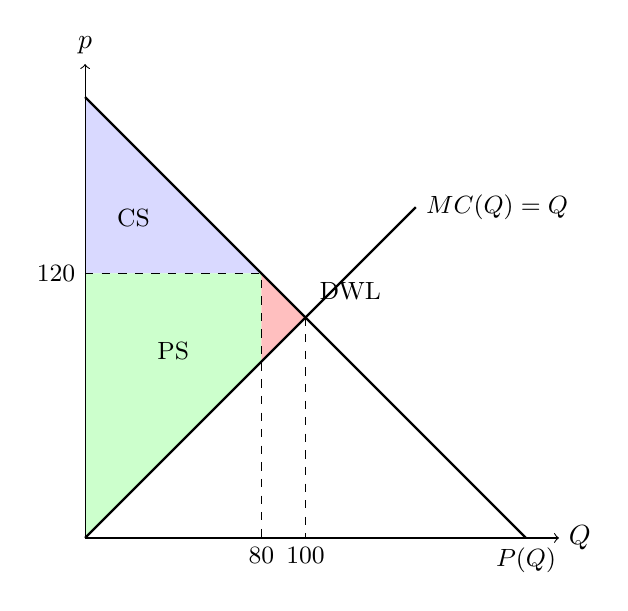
\begin{tikzpicture}[scale=0.028]
\fill[blue!15] (0,200)--(0,120)--(80,120)--cycle;
\fill[green!20] (0,0)--(0,120)--(80,120)--(80,80)--cycle;
\fill[red!25] (80,120)--(80,80)--(100,100)--cycle;
\draw[->] (0,0)--(215,0) node[right]{$Q$};
\draw[->] (0,0)--(0,215) node[above]{$p$};
\draw[thick] (0,200)--(200,0) node[below]{\small $P(Q)$};
\draw[thick] (0,0)--(150,150) node[right]{\small $MC(Q)=Q$};
\draw[dashed] (0,120)--(80,120)--(80,0);
\draw[dashed] (100,100)--(100,0);
\node[left] at (0,120){\small 120};
\node[below] at (80,0){\small 80};
\node[below] at (100,0){\small 100};
\node at (22,145){\small CS};
\node at (40,85){\small PS};
\node[right] at (102,112){\small DWL};
\end{tikzpicture}
\end{center}
\end{solution}
\item[4.6] Explain why the Cournot outcome is not efficient.
\begin{solution}
When firm $i$ increases output it lowers the price on \emph{all} units sold, including its rival's. Firm $i$ counts only the loss on its own units ($P'(Q)q_i$), so it ignores the harm to its rival. Each firm restricts quantity to keep the price high and capture more of the gains from trade. The market underproduces ($80<100$), and trades worth more to buyers than they cost to produce do not happen. That loss is the DWL. Like the Prisoner's Dilemma, this is a NE that is not Pareto efficient for society.
\end{solution}
\item[4.7] Now suppose there are $n$ identical firms, each with $C(q_i)=q_i^2$. Find the best response $b_i(Q_{-i})$, the symmetric Cournot quantity $q^c(n)$ and price $p^c(n)$. What happens as $n\to\infty$?
\begin{solution}
$\pi_i=(200-q_i-Q_{-i})q_i-q_i^2$. The FOC $200-4q_i-Q_{-i}=0$ gives $b_i(Q_{-i})=(200-Q_{-i})/4$. With symmetry, $Q_{-i}=(n-1)q$, so $4q=200-(n-1)q$ and
\[q^c(n)=\frac{200}{n+3},\qquad Q^c(n)=\frac{200n}{n+3},\qquad p^c(n)=\frac{600}{n+3}.\]
Check: $n=2$ gives $q^c=40$, $p^c=120$. As $n\to\infty$, $Q^c\to200$ and $p^c\to0$. Each firm becomes tiny, so its marginal cost $2q^c\to0$ and price converges to marginal cost: the competitive, efficient outcome.
\end{solution}
\end{description}

\end{document}
